% Title page
\frame[plain]{\titlepage}

\lecture{Введение}{intro}

\section{Факты, правила и запросы}
\subsection{Основные пункты}

\begin{frame}
	\frametitle{\insertsection}
	\framesubtitle{\insertsubsection}
	\begin{itemize}
		\item Рассмотреть простые примеры программ на \textbf{Prolog}, определить понятия факта, правила, запроса и базы знаний
		\item Дать определения основных понятий и синтаксических конструкций, таких как атомы, переменные и термы
	\end{itemize}
\end{frame}

\subsection{База знаний}

\begin{frame}
	\frametitle{\insertsection}
	\framesubtitle{\insertsubsection}
	Базовые конструкции языка \textbf{Prolog}:
	\begin{itemize}
		\item Факты
		\item Правила
		\item Запросы
	\end{itemize}
	Программа на Prolog представляет собой множество \textbf{фактов} и \textbf{правил}~--- \alert{Базу Знаний}
	Чтобы использовать информацию, содержащуюся в базе знаний, необходимо ставить \textbf{запросы}.
\end{frame}

\begin{frame}
	\frametitle{\insertsection}
	\framesubtitle{\insertsubsection}
	Пример 1
	
	
	\texttt{\begin{itemize}
				\item[] woman(mia).
				\item[] woman(jody).
				\item[] woman(yolanda).
				\item[] playsGuitar(jody).
				\item[]<2-> listensToMusic(mia).
				\item[]<2-> musician(yolanda).
				\item[]<2-> playsGuitar(mia) :- listensToMusic(mia).
				\item[]<2-> playsGuitar(yolanda) :- listensToMusic(yolanda).
				\item[]<2-> listensToMusic(yolanda) :- musician(yolanda).
			\end{itemize}}
\end{frame}

\begin{frame}
	\frametitle{\insertsection}
	\framesubtitle{\insertsubsection}
	Пример 2
	
	
	\texttt{\begin{itemize}
		\item[] musician(mia).
		\item[] listensToMusic(jody).
		\item[] playsGuitar(mia) :- listensToMusic(mia),musician(mia).
		\item[] playsGuitar(jody) :- musician(jody); listensToMusic(jody).
	\end{itemize}}
\end{frame}

\begin{frame}
	\frametitle{\insertsection}
	\framesubtitle{\insertsubsection}
	Пример 3
	
	
	\texttt{\begin{itemize}
		\item[] woman(mia).
		\item[] woman(jody).
		\item[] woman(yolanda).
		\item[] loves(vincent,mia).
		\item[] loves(marcellus,mia).
	\end{itemize}}
\end{frame}

\begin{frame}
	\frametitle{\insertsection}
	\framesubtitle{\insertsubsection}
	Пример 4
	
	
	\texttt{\begin{itemize}
			\item[] loves(vincent,mia).
			\item[] loves(marcellus,mia).
			\item[] jealous(X,Y) :- loves(X,Z),loves(Y,Z).
	\end{itemize}}
\end{frame}

\subsection{Синтаксис}

\begin{frame}
	\frametitle{\insertsection}
	\framesubtitle{\insertsubsection}
	\textbf{\underline{Атомы}}
	
	\begin{enumerate}
		\item Последовательность строчных или прописных букв, цифр и символов подчерка, начинающаяся со строчной буквы.
		\item Произвольная последовательность символов, заключённая в одинарные кавычки.
		\item Последовательность спецсимволов.
	\end{enumerate}

	\begin{rexample}
		mia, marcellus, big\_kahuna\_burger, 'Произвольная строка символов', ====>, :-
	\end{rexample}
\end{frame}

\begin{frame}
	\frametitle{\insertsection}
	\framesubtitle{\insertsubsection}
	\textbf{\underline{Числа}}
	
	\begin{enumerate}
		\item Действительные числа: 2,718; 103,3087; \(\pi \), \ldots
		\item Целые числа: -2, -1, 0, 1, 2, \ldots
	\end{enumerate}

	\textbf{\underline{Переменные}}
	
	
	\textbf{Переменные} служат для обозначения объектов, значения которых меняются в ходе выполнения программы. Имя переменной задается
	последовательностью строчных или прописных букв, цифр и символов подчерка, начинающейся с \textbf{прописной буквы} или \textbf{символа подчерка}.
	
	\begin{rexample}
		X, Y, Variable, \_X, X1, \_variable\_with\_some\_info\_
	\end{rexample}
\end{frame}

\begin{frame}
	\frametitle{\insertsection}
	\framesubtitle{\insertsubsection}
	\textbf{\underline{Термы}}
	
	\textit{Терм (составной терм)} состоит из \alert{функтора} и последовательности аргументов в скобках.
	\begin{enumerate}
		\item Любой атом или число является термом. Такие термы называются \alert{константами}.
		\item Любая переменная является термом.
		\item Имя функтора~--- это атом.
		\item Переменная не может быть функтором.
		\item Аргументы составного терма должны быть термами.
	\end{enumerate}

	\begin{rexample}
		loves(vincent, mia), playsGuitar(jody), jody, musician(mia), eats(cat,Prey)
	\end{rexample}
\end{frame}

\subsection{Проверочные вопросы}

\begin{frame}
	\frametitle{\insertsection}
	\framesubtitle{\insertsubsection}
	Какие из перечисленных строк являются атомами, какие переменными, а какие не являются ни тем, ни другим?
	\texttt{\begin{enumerate}
		\item vINCENT
		\item Foot
		\item x1
		\item Y3
		\item big\_kahuna\_burger
		\item 'Криминальное чтиво'
		\item roast chicken
		\item \_IndianaJones
		\item '\_IndianaJones'
	\end{enumerate}}
\end{frame}

\begin{frame}
	\frametitle{\insertsection}
	\framesubtitle{\insertsubsection}
	Какие из перечисленных ниже строк являются атомами, переменными или составными термами, а какие вообще не являются термами? Для каждого составного терма укажите имя функтора и его арность.
	\texttt{\begin{enumerate}
		\item loves(vincent,mia)
		\item 'loves(vincent,mia)'
		\item Eats(cat,mouse)
		\item hasChildren(cat,kittens)
		\item and(musician(jody),artist(mia))
		\item and(musician(X),artist(Y))
		\item \_and(musician(jody),artist(mia))
		\item (Butch kills Vincent)
		\item kills(Butch,Vincent)
		\item kills(Butch,Vincent
	\end{enumerate}}
\end{frame}

\begin{frame}
	\frametitle{\insertsection}
	\framesubtitle{\insertsubsection}
	Сколько фактов, правил, высказываний и предикатов в следующей базе знаний? Для каждого правила назовите вывод и цели.
	\texttt{\begin{itemize}
			\item[] woman(mia).
			\item[] woman(jody).
			\item[] man(jules).
			\item[] person(X) :- man(X); woman(X).
			\item[] loves(X,Y) :- knows(Y,X).
			\item[] father(Y,Z) :- man(Y), son(Z,Y).
			\item[] father(Y,Z) :- man(Y), daughter(Z,Y).
	\end{itemize}}
\end{frame}

\subsection{Упражнения}

\begin{frame}
	\frametitle{\insertsection}
	\framesubtitle{\insertsubsection}
	Запишите следующую базу знаний на языке Prolog.
	
	\begin{itemize}
		\item Бутч убийца.
		\item Миа и Марселлас женаты.
		\item Зед мертв.
		\item Марселлас убьет любого, кто сделает Мие массаж стопы.
		\item Миа любит любого, кто хорошо танцует.
		\item Джулс ест все, что вкусно или питательно.
	\end{itemize}
\end{frame}

\begin{frame}
	\frametitle{\insertsection}
	\framesubtitle{\insertsubsection}
	Пусть дана следующая база знаний:
	\texttt{\begin{itemize}
			\item[] sportsman(john).
			\item[] hasUniform(harry).
			\item[] footballPlayer(harry).
			\item[] sportsman(X) :- isTrained(X),hasUniform(X).
			\item[] isTrained(X) :- footballPlayer(X).
	\end{itemize}}
	
	Как Prolog ответит на следующие запросы?
	\texttt{\begin{enumerate}
			\item sportsman(john).
			\item footballPlayer(john).
			\item sportsman(harry).
			\item sportsman(X).
			\item hockeyPlayer(john).
	\end{enumerate}}
\end{frame}

\subsection{Дополнительное задание}

\begin{frame}
	\frametitle{\insertsection}
	\framesubtitle{\insertsubsection}
	Средствами языка Prolog \textbf{определить, какие животные не имеют хозяина.}
	\begin{enumerate}
		\item Бутси~--- коричневая кошка.
		\item Корни~--- черная кошка.
		\item Мак~--- рыжая кошка.
		\item Флэш, Ровер и Спот~--- собаки, Ровер~--- рыжая, а Спот~--- белая.
		\item Все животные, которыми владеют Том и Кейт, имеют родословные.
		\item Том владеет всеми черными и коричневыми животными, а Кейт владеет всеми собаками небелого цвета, которые не являются собственностью Тома.
		\item Алан владеет Мак, если Кейт не владеет Бутси и если Спот не имеет родословной.
		\item Флэш~--- пятнистая собака.
	\end{enumerate}
\end{frame}

\lecture{Matching}{match}

\section{Унификация термов и поиск решений}
\subsection{Основные пункты}

\begin{frame}
	\frametitle{\insertsection}
	\framesubtitle{\insertsubsection}
	\begin{itemize}
		\item Познакомиться с понятием согласования термов.
		\item Разобраться в стратегиях, используемых интерпретатором языка Prolog для поиска ответов на вопросы.
	\end{itemize}
\end{frame}

\subsection{Определение}

\begin{frame}
	\frametitle{\insertsection}
	\framesubtitle{\insertsubsection}
	\only<1>{Два терма \alert{унифицированы}, если они равны или если они содержат переменные и существует означивание этих переменных, такое, что термы становятся равными.}
	\only<2->{\begin{enumerate}
			\item Если \texttt{term1} и \texttt{term2} константы, то \texttt{term1} и \texttt{term2} унифицированы тогда и только тогда, когда они равны друг другу, т.е. \texttt{term1} и \texttt{term2} это один и тот же атом или число.
			\item Если \texttt{term1}~--- это переменная, а \texttt{term2}~--- любой терм, то термы \texttt{term1} и \texttt{term2} унифицированы, и переменная \texttt{term1} инициализируется значением терма \texttt{term2}. 
			Если \texttt{term1} и \texttt{term2}~--- переменные, они унифицированы и принимают значения друг друга. Говорят, что переменные \texttt{term1} и \texttt{term2} \alert{разделяют значение}.
			\item Если \texttt{term1} и \texttt{term2} составные термы, то они унифицированы тогда и только тогда, когда:
			\begin{enumerate}[(a)]
				\item Их функторы и арность совпадают.
				\item Соответствующие аргументы обоих термов унифицированы. При этом означивание переменных согласовано.
			\end{enumerate}
			\item Два терма унифицированы тогда и только тогда, когда это следует из одного из предыдущих пунктов.
	\end{enumerate}}
\end{frame}

\subsection{Примеры унификации}

\begin{frame}
	\frametitle{\insertsection}
	\framesubtitle{\insertsubsection}
	\textbf{Какие из термов унифицированы?}
	\texttt{\begin{itemize}
		\item john = john.
		\item 42 = 42.
		\item 'Строка слов' = 'Строка слов'.
		\item 'mia' = mia.
		\item '42' = 42.
		\item mia = X.
		\item X = Y.
		\item kill(shoot(gun),Y) = kill(X,stab(knife)).
		\item loves(X,X) = loves(marcellus,mia).
		\item parent(A) = A.
	\end{itemize}}
\end{frame}

\subsection{Поиск решений}

\begin{frame}
	\frametitle{\insertsection}
	\framesubtitle{\insertsubsection}
	Интерпретатор языка Prolog обрабатывает условия запроса последовательно слева направо. Для каждого из условий интерпретатор ищет унифицируемый с ним факт или вывод правила, проходя базу знаний сверху вниз.
\end{frame}

\begin{frame}
	\frametitle{\insertsection}
	\framesubtitle{\insertsubsection}
	\texttt{\begin{itemize}
			\item[] person(vincent).
			\item[] person(jules).
			\item[] hasGun(vincent).
			\item[] hasGun(jules).
			\item[] alive(jules).
			\item[] lucky(X) :- person(X),hasGun(X),alive(X).
	\end{itemize}}
\end{frame}

\subsection{Дерево поиска решений}

\begin{frame}
	\frametitle{\insertsection}
	\framesubtitle{\insertsubsection}
	\begin{figure}
		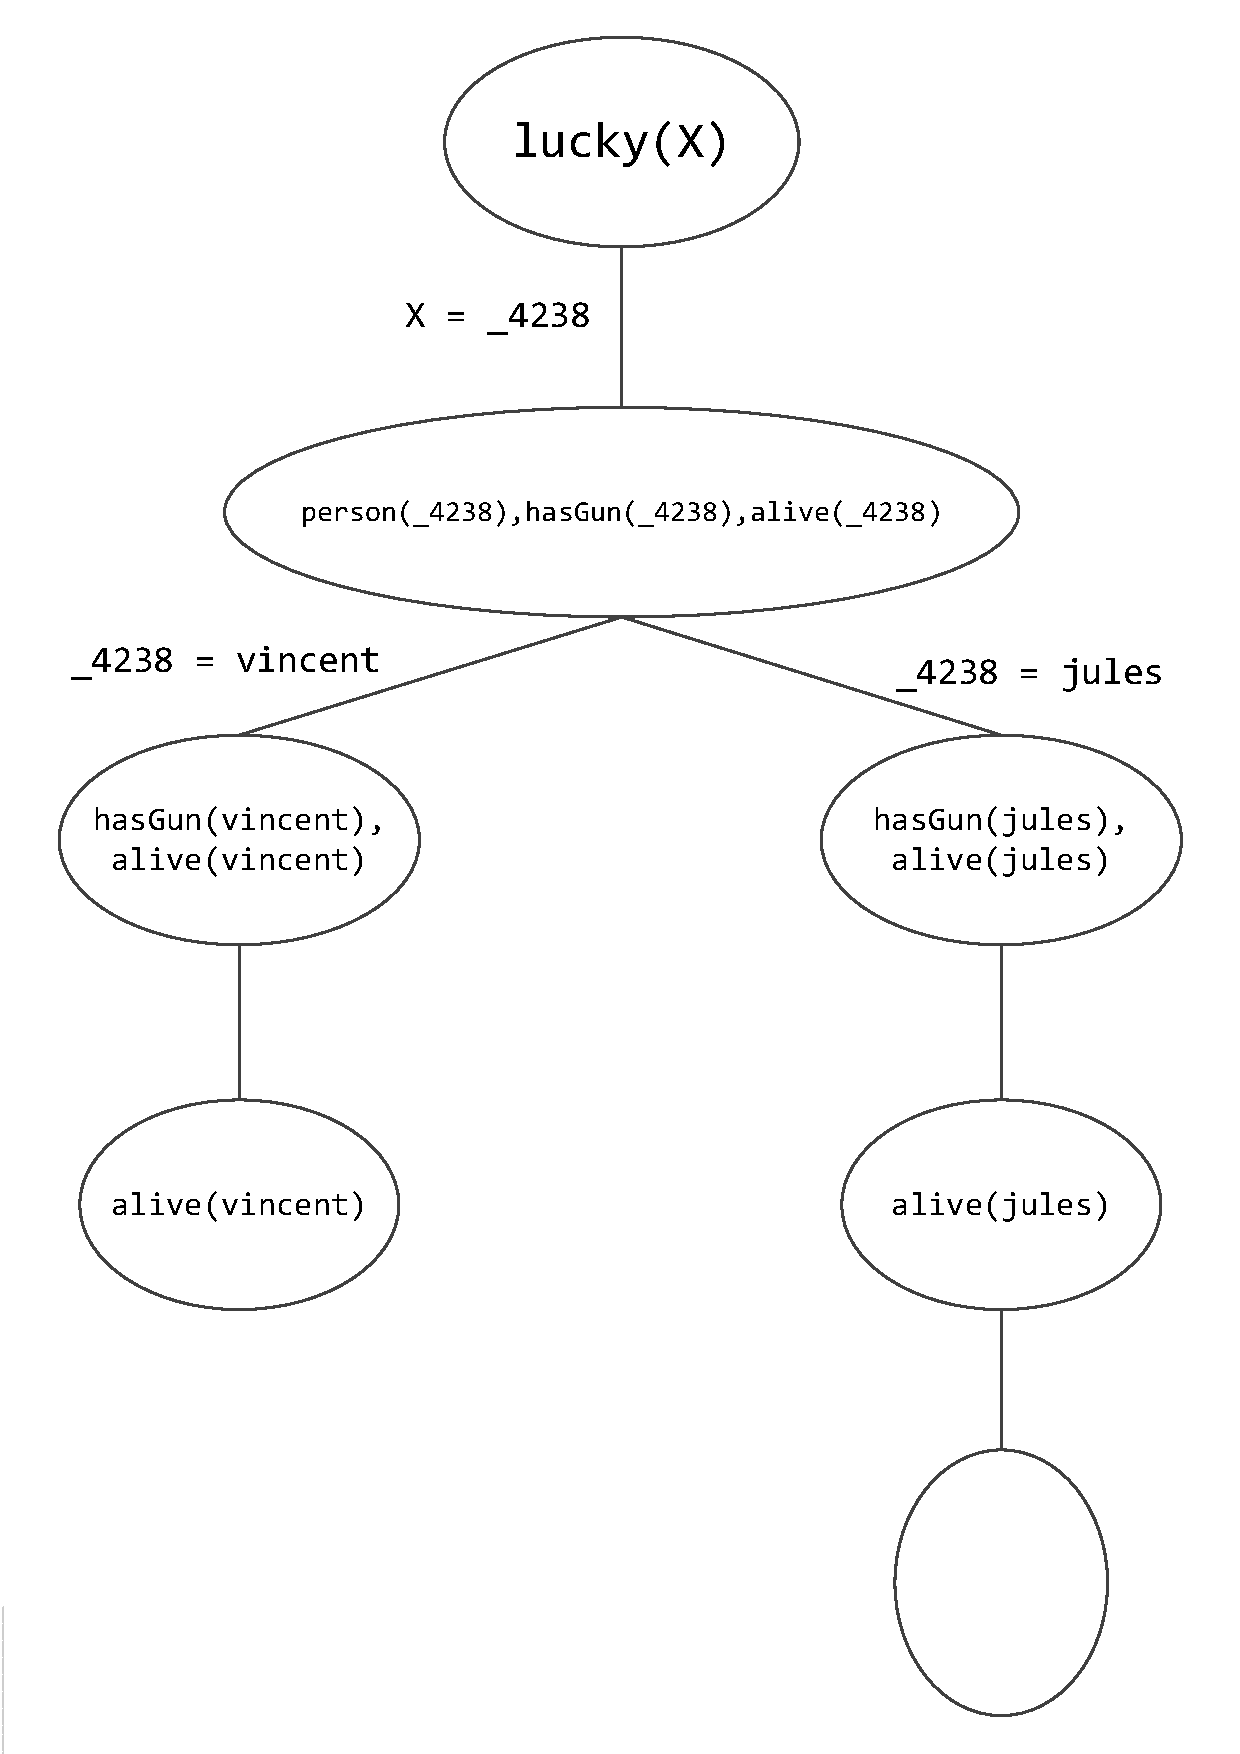
\includegraphics[scale=0.35]{stree}
	\end{figure}
\end{frame}

\subsection{Упражнения}

\begin{frame}
	\frametitle{\insertsection}
	\framesubtitle{\insertsubsection}
	В каких из перечисленных пар термы унифицированы? Где необходимо запишите значения переменных, необходимые для унификации.
	\texttt{\begin{enumerate}
			\item bread = bread.
			\item 'Bread' = bread.
			\item 'bread' = bread.
			\item Bread = bread.
			\item хлеб = котлета.
			\item food(bread) = bread.
			\item food(bread) = Bread.
			\item food(Bread) = food(bread).
			\item food(хлеб,X) = food(Y,котлета).
			\item graph(edge(v1,v2),X,edge(Y,v4)) = graph(Z,edge(v7,v8),edge(v4,X)).
			\item food(X) = X.
			\item meal(food(bread),drink(beer)) = meal(food(X),Y).
			\item meal(food(bread),X) = meal(X,drink(beer)).
	\end{enumerate}}
\end{frame}

\begin{frame}
	\frametitle{\insertsection}
	\framesubtitle{\insertsubsection}
	\textbf{Пусть дана следующая база знаний.}
	\texttt{\begin{itemize}
			\item[] witch(gullveig).
			\item[] god(freyja).
			\item[] god(odin).
			\item[] god('Vidarr').
			\item[] magic(X) :- witch(X).
			\item[] magic(X) :- wizard(X).
			\item[] magic(X) :- god(X).
	\end{itemize}}
	\textbf{Каким из запросов она удовлетворяет?}
	\texttt{\begin{enumerate}
			\item magic(witch).
			\item wizard(odin).
			\item magic('Vidarr').
			\item magic(Vidarr).
	\end{enumerate}}
\end{frame}

\begin{frame}
	\frametitle{\insertsection}
	\framesubtitle{\insertsubsection}
	\textbf{Дан следующий лексикон.}
	\texttt{\begin{itemize}
			\item[] word(article,a).
			\item[] word(article,every).
			\item[] word(noun,criminal).
			\item[] word(noun,'big kahuna burger').
			\item[] word(verb,eats).
			\item[] word(verb,likes).
%			\item[] sentence(W1,W2,W3,W4,W5) :- word(article,W1), word(noun,W2), word(verb,W3), word(article,W4), word(noun,W5).
	\end{itemize}}
	Написать запрос на получение списка всех возможных фраз данного лексикона, имеющих вид: \textit{артикль+существительное+глагол+артикль+существительное}. Построить дерево поиска решений для одной из построенных фраз.
\end{frame}

\begin{frame}
	\frametitle{\insertsection}
	\framesubtitle{\insertsubsection}
	Имеется следующий список слов: \textit{бок, акр, сомо, бокс, хата, эдда, вино, рода, окот, анод, скала, онагр, обиход, монако, дверка, дигора, удокан, маарри, бинокль, бегония}.
	Пусть в базе знаний слова представляются следующим образом:
	\texttt{\begin{itemize}
			\item[] word(эдда,э,д,д,а).
			\item[] word(вино,в,и,н,о).
			\item[] word(рода,р,о,д,а).
			\item[] word(окот,о,к,о,т).
			\item[] word(анод,а,н,о,д).
			\item[] word(скала,с,к,а,л,а).
			\item[] word(онагр,о,н,а,г,р).
			\item[] word(обиход,о,б,и,х,о,д).
	\end{itemize}}
\end{frame}

\begin{frame}
	\frametitle{\insertsection}
	\framesubtitle{\insertsubsection}
	Реализовать предикат \texttt{crosswd/10 = crosswd(V1,V2,V3,V4,V5,V6,H1,H2,H3,H4)}, который бы заполнял данными словами следующий кроссворд таким образом, чтобы
	слова, идущие вертикально, были первыми 6 аргументами, а слова, идущие горизонтально~--- последними.
	\begin{figure}
		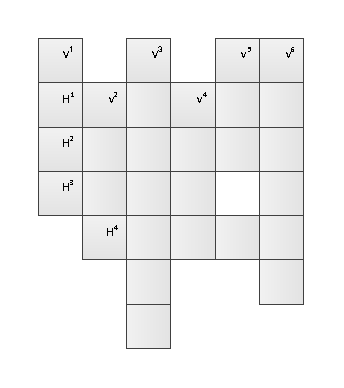
\includegraphics[scale=0.9]{crosswd}
	\end{figure}
\end{frame}

\lecture{Recursion}{recursion}

\begin{frame}[plain,c]

	\begin{center}
		\Huge Определения и примеры
	\end{center}

\end{frame}

\section{Рекурсия в Prolog}
\subsection{Простой пример}

\begin{frame}
	\frametitle{\insertsection}
	\framesubtitle{\insertsubsection}
	\texttt{\begin{itemize}
			\item[] переваривает(Хищник,Добыча) :- съел(Хищник,Добыча).
			\item[] переваривает(Хищник,Добыча) :- съел(Хищник,ДругойХищник), переваривает(ДругойХищник,Добыча).
			\item[] съел(комар,кровь).
			\item[] съел(лягушка, комар).
			\item[] съел(цапля, лягушка).
	\end{itemize}}
\end{frame}

\section{Уровни понимания программ}
\subsection{Декларативный и процедурный}

\begin{frame}
	\frametitle{\insertsection}
	\framesubtitle{\insertsubsection}
	\alert{Декларативный смысл} Prolog-программы касается только \textit{отношений}, определенных в программе.
	Другими словами, декларативный смысл определяет, что должно быть результатом работы программы с точки зрения математической логики.
	
	\alert{Процедурный смысл} программы определяет еще и как этот результат был получен, т.е. как отношения реально обрабатываются пролог-системой.
\end{frame}

\section{Правила описания рекурсивных предикатов}
\subsection{База и шаг рекурсии}

\begin{frame}
	\frametitle{\insertsection}
	\framesubtitle{\insertsubsection}
	\only<1>{\textbf{База рекурсии}}
	\only<2>{\textbf{Шаг рекурсии}}
	
	
	\texttt{\begin{itemize}
			\item[] {\color<1>[RGB]{0,0,255}{переваривает(Хищник,Добыча) :- съел(Хищник,Добыча).}}
			\item[] {\color<2>[RGB]{0,0,255}{переваривает(Хищник,Добыча) :- съел(Хищник,ДругойХищник), переваривает(ДругойХищник,Добыча).}}
			\item[] съел(комар,кровь).
			\item[] съел(лягушка, комар).
			\item[] съел(цапля, лягушка).
	\end{itemize}}
\end{frame}

\subsection{descending.pl}

\begin{frame}
	\frametitle{\insertsection}
	\framesubtitle{\insertsubsection}
	\texttt{\begin{itemize}
			\item[] child(adam,cain).
			\item[] child(adam,abel).
			\item[] child(adam,seth).
			\item[] child(cain,enoch).
			\item[] child(enoch,irad).
			\item[] child(irad,mehujael).
			\item[] child(seth,enos).
			\item[] child(enos,kenan).
			\item[] child(kenan,mahalalel).
			\item<2->[] descend(A,D) :- child(A,D).
			\item<2->[] descend(A,D) :- child(A,C), descend(C,D).
	\end{itemize}}
\end{frame}

\subsection{arithmetic.pl}

\begin{frame}
	\frametitle{\insertsection}
	\framesubtitle{\insertsubsection}
	\texttt{\begin{itemize}
			\item[] num(0).
			\item[] num(s(N)) :- num(N).
			\item<2->[] plus(0,N,N).
			\item<2->[] plus(s(M),N,s(Sum)) :- plus(M,N,Sum).
	\end{itemize}}
\end{frame}

\section{Рекурсия и хвостовая рекурсия}
\subsection{Численная арифметика: вычисление факториала числа}

\begin{frame}
	\frametitle{\insertsection}
	\framesubtitle{\insertsubsection}
	
	\texttt{\begin{itemize}
			\item[] f(0,1).
			\item[] f(X,Y) :- X>0,X1 is X-1,f(X1,Y1),Y is Y1*X.
	\end{itemize}}

	\uncover<2->{\texttt{\begin{itemize}
				\item[] f(N,N,F):-write(F),!.
				\item[] f(N,N1,F1):- N2 is N1+1,F2 is F1*N2,f(N,N2,F2).
				\item[] factorial(N):- f(N,1,1).
	\end{itemize}}}

\end{frame}

\section{Последовательность целей и остановка программ}
\subsection{Возможные источники ошибок}

\begin{frame}

	\frametitle{\insertsection}
	\framesubtitle{\insertsubsection}
	\texttt{\begin{itemize}
			\item[] child(adam,cain).
			\item[] child(adam,abel).
			\item[] child(adam,seth).
			\item[] child(cain,enoch).
			\item[] child(enoch,irad).
			\item[] child(irad,mehujael).
			\item[] child(seth,enos).
			\item[] child(enos,kenan).
			\item[] child(kenan,mahalalel).
	\end{itemize}}
	\texttt{\only<1>{\begin{itemize}
				\item[] descend(A,D) :- child(A,D).
				\item[] descend(A,D) :- child(A,C), descend(C,D).
			\end{itemize}}
		\only<2>{\begin{itemize}
				\item[] descend(A,D) :- descend(C,D), child(A,C).
				\item[] descend(A,D) :- child(A,D).
		\end{itemize}}
		\only<3>{\begin{itemize}
				\item[] descend(A,D) :- child(A,D).
				\item[] descend(A,D) :- descend(C,D), child(A,C).
		\end{itemize}}
		\only<4>{\begin{itemize}
				\item[] descend(A,D) :- child(A,C), descend(C,D).
				\item[] descend(A,D) :- child(A,D).
		\end{itemize}}
	}

\end{frame}

\begin{frame}

	\frametitle{\insertsection}
	\framesubtitle{\insertsubsection}
	
	\texttt{\begin{itemize}
			\item[] num(0).
			\item[] num(s(N)) :- num(N).
		\end{itemize}
	}
	
	\texttt{\begin{itemize}
			\item[] num(s(N)) :- num(N).
			\item[] num(0).
		\end{itemize}
	}

\end{frame}

\begin{frame}[plain,c]

	\begin{center}
		\Huge Упражнения
	\end{center}

\end{frame}


\section{Упражнения}

\begin{frame}
	\frametitle{\insertsection}
	\begin{itemize}
		\item Скачайте или перепишите листинг программы \texttt{descending.pl}. Рассмотрите каждый случай рекурсии (см. слайды ранее). Какие запросы работают, какие нет? Почему?
		\item Скачайте или перепишите листинг программы \texttt{arithmetic.pl}. Реализуйте следующие операции над числами, определенными в программе:
		\begin{enumerate}
			\item \textbf{Умножение}: реализуйте предикат \texttt{times/3}, такой, чтобы последним аргументом было произведение двух первых.
			\item \textbf{Возведение в степень}: реализуйте предикат \texttt{exp(N,X,R)}, такой, чтобы \(R = X^{N}\).
			\item \textbf{Сравнение}: реализуйте предикаты \texttt{gt/2, lt/2}, истинные тогда, когда первый аргумент больше (меньше), чем второй.
			\item \textbf{Равенство}: реализуйте предикат \texttt{eq/2}, истинный тогда и только тогда, когда его аргументы равны.
			\item \textbf{Максимум и минимум двух чисел}: реализуйте предикаты \texttt{max/3, min/3}, где третий аргумент~--- это максимум (минимум) из двух первых.
		\end{enumerate}
	\end{itemize}
\end{frame}

\begin{frame}
	\frametitle{\insertsection}
	\begin{itemize}
		\item Реализуйте программу для вычисления факториала числа (в обычной численной арифметике). Сравните время работы и количество операций в зависимости от значения входных параметров.
		\item Реализуйте программу для вычисления чисел Фибоначчи. Реализуйте предикат \texttt{getFibN/2 = getFibN(N, Fn)}, такой, что \(F_n\)~--- N-е число Фибоначчи.
		\item Используя предыдущую программу, реализуйте предикат \texttt{getNearestFibonacci/3}, возвращающий по заданному числу номер ближайшего к нему числа Фибоначчи и его номер.
	\end{itemize}
\end{frame}



\lecture{Additional Excercises}{recursionExt}

\section{Дополнительные упражнения}

\begin{frame}
	
	\frametitle{\insertsection}
	
	Преобразуйте программу \texttt{arithmetic.pl}.
	
	\begin{itemize}
		\item Реализуйте операцию деления \(N\) на \(M\) с остатком таким образом, чтобы результатом были два числа \(Q\) и \(P\), такие, что \(N = M\cdot Q + P \).
		\item Реализуйте алгоритм Евклида для поиска наибольшего общего делителя двух заданных чисел.
	\end{itemize}
	
\end{frame}

\begin{frame}
	\frametitle{\insertsection}
	Опишите следующий граф в виде базы знаний. Реализуйте предикат \texttt{fromTo/2 = fromTo(Begin,End)}, который по заданным началу и концу маршрута будет выяснять, существует ли путь между
	заданными вершинами и печатать в консоли слово, которое получается при следовании по найденному пути.
	
	\begin{figure}
		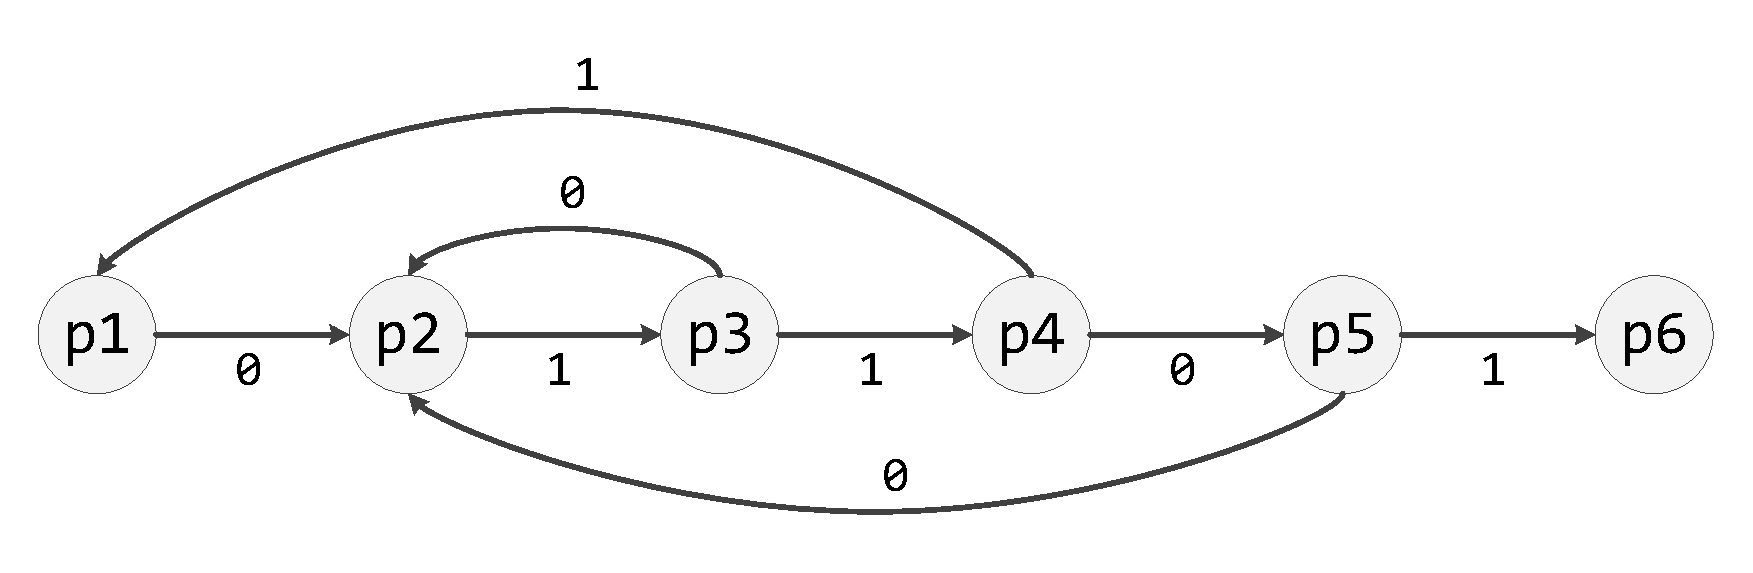
\includegraphics[scale=0.35]{graph}
	\end{figure}
\end{frame}

\begin{frame}[shrink=7]
	\frametitle{\insertsection}
	Скачайте базу знаний \texttt{travel.pl} или перепишите.
	\texttt{\begin{itemize}
		\item[] byCar(auckland,hamilton).
		\item[] byCar(hamilton,raglan).
		\item[] byCar(valmont,saarbruecken).
		\item[] byCar(valmont,metz).
		\item[] byTrain(metz,frankfurt).
		\item[] byTrain(saarbruecken,frankfurt).
		\item[] byTrain(metz,paris).
		\item[] byTrain(saarbruecken,paris).
		\item[] byPlane(frankfurt,bangkok).
		\item[] byPlane(frankfurt,singapore).
		\item[] byPlane(paris,losAngeles).
		\item[] byPlane(bangkok,auckland).
		\item[] byPlane(losAngeles,auckland).
	\end{itemize}}
	Реализуйте предикат \texttt{travel/2}, который по заданным началу и концу маршрута определял бы, существует ли способ добраться из начала в конец и
	печатал пункты маршрута, а также виды транспорта, которыми осуществляется перемещение между промежуточными пунктами.
\end{frame}

\begin{frame}
	
	\frametitle{\insertsection}
	
	Реализуйте некоторый каталог вида \texttt{unit(key, value)}. Например, список книг по авторам:
	\texttt{\begin{itemize}
			\item[] book(heinlein, 'Stranger in a Strange Land').
			\item[] book(heinlein, 'The Moon Is a Harsh Mistress').
			\item[] book(niven, 'Lucifer's Hammer').
	\end{itemize}}
	
	Реализуйте программу, запрашивающую из консоли ввод автора и печатающая либо список его книг, либо сообщение, что книг данного автора в каталоге нет.
	
\end{frame}

\lecture{Lists}{lists}

\begin{frame}[plain,c]

	\begin{center}
		\Huge Понятие и вид списка в Prolog
	\end{center}

\end{frame}

\section{Списки}

\subsection{Список в Prolog}

\begin{frame}
	\frametitle{\insertsection}
	\framesubtitle{\insertsubsection}
	
	\begin{itemize}
		\item Списком называют конечную последовательность элементов.
		\item В синтаксисе языка Prolog границы списка определяются квадратными скобками [ и ].
		\item Элементы списка отделяются друг от друга запятой. Элементами списка могут быть любые термы.
		\item Любой непустой список можно разделить на голову и хвост (head и tail). Для записи используется специальный символ |. 
		\texttt{[Head | Tail] = [one, two, three]} => \texttt{Head = one, Tail = [two, three]}. Голова списка~--- это элемент,
		хвост списка~--- это список.
		\item Пустой список не может быть разделен на голову и хвост.
	\end{itemize}

\end{frame}

\subsection{Простой пример}

\begin{frame}

	\frametitle{\insertsection}
	\framesubtitle{\insertsubsection}
	
	\texttt{\begin{itemize}
			\item[] []
			\item[] [first, second, third, fourth, fifth]
			\item[] [1, 2, 3, 4, 5, 6, 7, 8, 9, 0]
			\item[] [first, 2, color(cornie, black), F, fifth, F]
			\item[] [first, second, [third, fourth], [fifth, color(cornie, black)]]
			\item[] [[], [], car(volkswagen), F, 1, 2, [1, F, car(bmw), [1, 2, 4]], X]
	\end{itemize}}

\end{frame}

\subsection{Получение элементов списка}

\begin{frame}

	\frametitle{\insertsection}
	\framesubtitle{\insertsubsection}
	
	\texttt{\begin{itemize}
			\item[] [abyssian, bobtail, [bengal, birman]]
	\end{itemize}}

	\texttt{\begin{itemize}
			\item<2-> {[H|T]} = [abyssian, bobtail, [bengal, birman]].
			\item<3-> {[F,S|T]} = [abyssian, bobtail, [bengal, birman]].
			\item<4-> {[\_,S|T]} = [abyssian, bobtail, [bengal, birman]].
			\item<5-> {[First,\_,\_,Fourth|\_]} = [abyssian, bobtail, [bengal, birman]].
			\item<6-> {[\_,\_,[\_|T]|\_]} = [abyssian, bobtail, [bengal, birman]].
	\end{itemize}}

\end{frame}

\section{Операции со списками}
\subsection{Проверка вхождения элемента}

\begin{frame}
	
	\frametitle{\insertsection}
	\framesubtitle{\insertsubsection}
	
	Предикат \alert{\texttt{member/2 = member(?Elem, ?List)}} имеет два аргумента~--- некоторый терм и список, и принимает значение \texttt{true} в
	случае, когда \texttt{?Elem} содержится в списке \texttt{?List}. В противном случае предикат принимает значение \texttt{false}.
	\newline \newline
	\uncover<2->{Как можно реализовать предикат \texttt{member/2} самостоятельно?}
	
	\texttt{\begin{itemize}
			\item<3->[] member(X, [X|T]).
			\item<4->[] member(X, [H|T]) :- member(X,T).
	\end{itemize}}

	\uncover<5->{\texttt{\begin{itemize}
				\item[] member(X, [X|\_]).
				\item[] member(X, [\_|T]) :- member(X,T).
	\end{itemize}}}
	
\end{frame}

\subsection{Разбор интересного примера}

\begin{frame}

	\frametitle{\insertsection}
	\framesubtitle{\insertsubsection}
	
	Какой-нибудь интересный пример на рекурсивный разбор списка или что-то в этом роде.

\end{frame}
